\documentclass[12pt,a4paper]{report}

% Packages
\usepackage[utf8]{inputenc}
\usepackage{setspace}
\usepackage{geometry}
\usepackage{hyperref}
\usepackage{graphicx}

\usepackage{tikz}
\usetikzlibrary{arrows.meta, calc, positioning, patterns}

\tikzstyle{block} = [draw, fill=white, rectangle, 
    minimum height=3em, minimum width=6em]
\tikzstyle{sum} = [draw, fill=white, circle, node distance=1cm]
\tikzstyle{input} = [coordinate]
\tikzstyle{output} = [coordinate]
\tikzstyle{pinstyle} = [pin edge={to-,thin,black}]

\onehalfspacing
\geometry{margin=1in}

\begin{document}

\title{Reducing the runtime of an NP-Hard algorithm using deep learning on historical data}
\author{Christoffer Lindkvist}
\date{\today}
\maketitle

\begin{abstract} 
    A mixed-model assembly line manufactures different product variants on a single line, where variations in tasks can create imbalances across workstations. When several labour-intensive models appear consecutively, some stations may exceed their capacity, leading to overloads. This challenge is formalized as the Product Sequencing Problem, an NP-hard optimization task concerned with arranging production orders into efficient sequences. This thesis investigates whether deep learning can complement heuristic methods for solving this problem. Using a deep learning model trained to emulate tacit scheduling knowledge captured in historical data, and using its predictions to initialize a heuristic algorithm. By providing informed starting points, this approach aims to reduce the computation time of the algorithm.
\end{abstract}

\chapter*{Acknowledgements} % the * avoids numbering
Funding: Vinnova grant 2023-00970 (EUREKA ITEA4 ArtWork), Vinnova grant 2023-00450 (Arrowhead fPVN, Swedish
funding), and KDT JU grant 2023-000450 (Arrowhead fPVN,
EU funding).


\tableofcontents

\chapter{Introduction}
\section{Background}
This thesis addresses the Product Sequencing Problem, an NP-Hard optimization problem arising in the planning of mixed-model assembly lines \cite{ref6}. Traditionally, product sequences are determined manually by management staff, relying primarily on tacit knowledge accumulated through experience. While this often produces feasible solutions with relatively few overlaps, it remains ad hoc and sporadic. %ad hoc = academic for "doohickey"

To improve upon this, a heuristic algorithm is proposed. The algorithm first generates a feasible baseline solution from pre-defined constraints, and then it refines the baseline until an acceptable sequence is reached. The central question of this thesis is whether the runtime of such an algorithm can be reduced by initializing it with a baseline informed by historical sequencing data, rather than relying solely on rule-based construction.

\section{Research Problem}
The Product Sequencing Problem is classified as NP-Hard. Current approaches in practice rely entirely on human expertise and tacit knowledge, which limits scalability and consistency. If this knowledge could be systematically emulated using a model that mimics historical sequencing data, and in effect tacit knowledge, it may provide stronger starting points for the heuristic methods. Such informed baselines could potentially reduce the runtime required to reach high-quality solutions, especially for complex sequencing instances.

\section{Objectives}
The objectives of this thesis are:
\begin{enumerate}
    \item To design a deep learning model capable of emulating the tacit knowledge of management workers using historical data.
    \item To integrate the model as a preprocessing step in the existing heuristic algorithm in order to reduce its runtime.
    \item To provide a visualization tool that intuitively illustrates the scheduling flow, highlighting overlaps, borrowed time, and bottlenecks across stations and time.
\end{enumerate}

\section{Visualization of the Problem}

The user interface (UI) will visualize the flow of the assembly line along two axes: one representing stations and one representing clockcycles. A clockcycle is defined as the time required for an item to move from one station to the next. In the visualization, items are displayed in a way that reflects the relative duration of processing at each station. In \autoref{fig:assembly}, this is illustrated by stretching items along the timeline to better represent the clockcycles. Note that a clockcycle is an arbitrary unit of time and does not correspond to real-world durations. For the purpose of this thesis, one clockcycle is defined as the time it takes for an arbitrary item $X$ to move from station $S_n$ to station $S_{n+1}$.

\begin{figure}[ht]
    \centering
    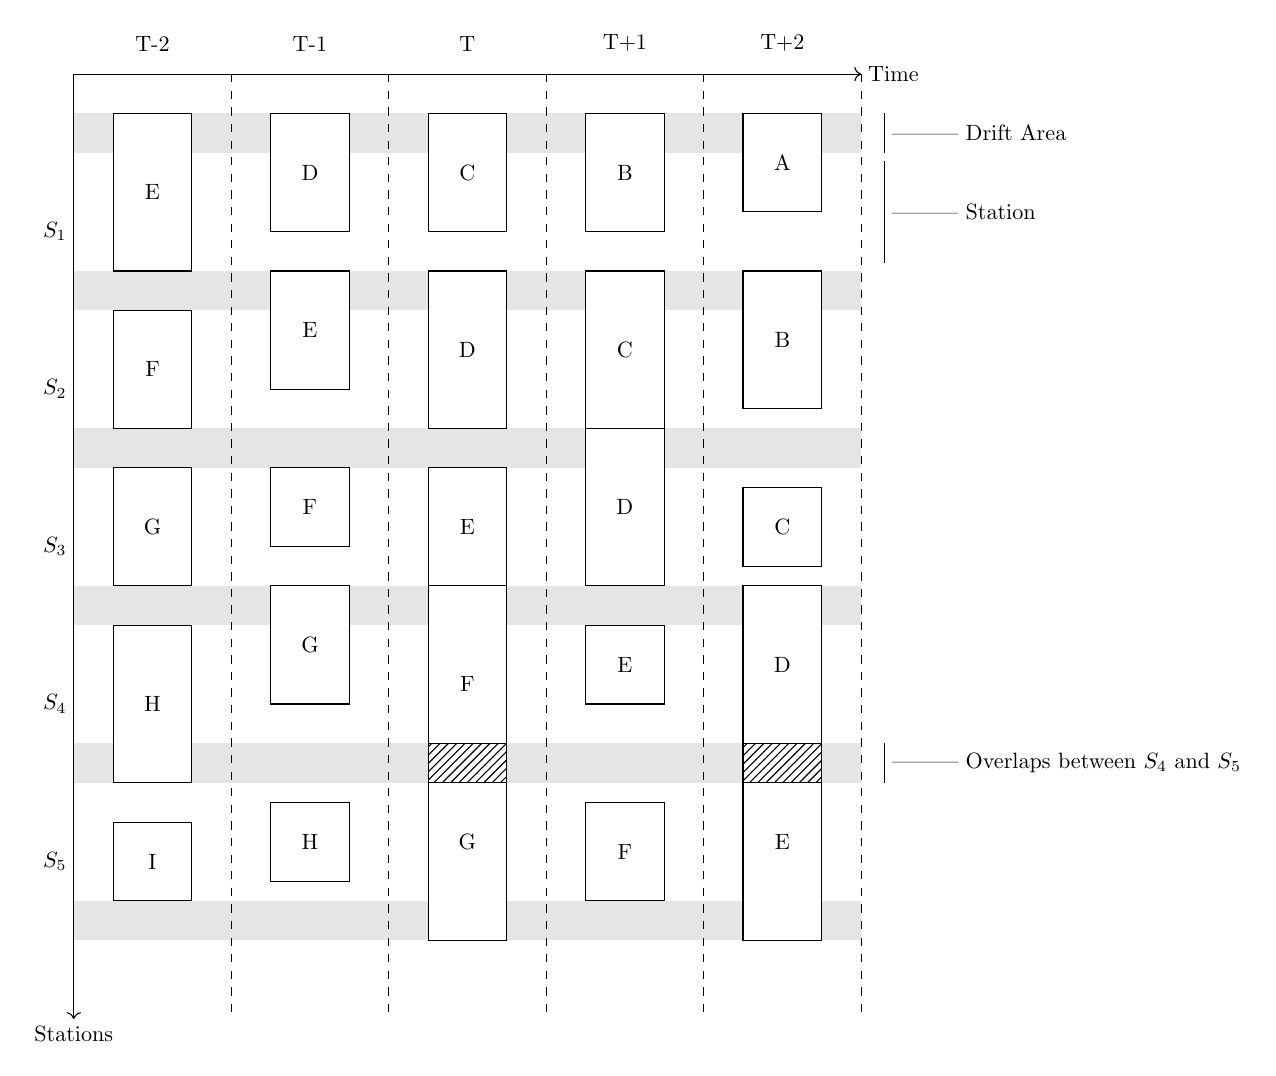
\begin{tikzpicture}[scale=1, every node/.style={scale=0.8, inner sep=3pt}]

        \foreach \y in {-1,-3,-5,-7,-9, -11} {
            \fill[gray!20] (0,\y+0.5) rectangle (10,\y);
        }

        \draw[->] (0,0) -- (10,0) node[right]{Time};
        \draw[->] (0,0) -- (0,-12) node[below]{Stations};

        \foreach \y/\name in { -2/$S_1$, -4/$S_2$, -6/$S_3$, -8/$S_4$, -10/$S_5$ } {
            \node[left] at (0,\y) { \name };
        }
        \draw[fill=white] (0.5,-9.5) rectangle (1.5,-10.5) node[midway]{I};

        \draw[fill=white] (0.5,-7) rectangle (1.5,-9) node[midway]{H};
        \draw[fill=white] (2.5,-9.25) rectangle (3.5,-10.25) node[midway]{H};

        \draw[fill=white] (0.5,-5) rectangle (1.5,-6.5) node[midway]{G};
        \draw[fill=white] (2.5,-6.5) rectangle (3.5,-8) node[midway]{G};
        \draw[fill=white] (4.5,-8.5) rectangle (5.5,-11) node[midway]{G};

        \draw[fill=white] (0.5,-3) rectangle (1.5,-4.5) node[midway]{F};
        \draw[fill=white] (2.5,-5) rectangle (3.5,-6) node[midway]{F};
        \draw[fill=white] (4.5,-6.5) rectangle (5.5,-9) node[midway]{F};
        \draw[fill=white] (6.5,-9.25) rectangle (7.5,-10.5) node[midway]{F};

        \draw[fill=white] (0.5,-0.5) rectangle (1.5,-2.5) node[midway]{E};
        \draw[fill=white] (2.5,-2.5) rectangle (3.5,-4) node[midway]{E};
        \draw[fill=white] (4.5,-5) rectangle (5.5,-6.5) node[midway]{E};
        \draw[fill=white] (6.5,-7) rectangle (7.5,-8) node[midway]{E};
        \draw[fill=white] (8.5,-8.5) rectangle (9.5,-11) node[midway]{E};

        \draw[fill=white] (2.5,-0.5) rectangle (3.5,-2) node[midway]{D};
        \draw[fill=white] (4.5,-2.5) rectangle (5.5,-4.5) node[midway]{D};
        \draw[fill=white] (6.5,-4.5) rectangle (7.5,-6.5) node[midway]{D};
        \draw[fill=white] (8.5,-6.5) rectangle (9.5,-8.5) node[midway]{D};

        \draw[fill=white] (4.5,-0.5) rectangle (5.5,-2) node[midway]{C};
        \draw[fill=white] (6.5,-2.5) rectangle (7.5,-4.5) node[midway]{C};
        \draw[fill=white] (8.5,-5.25) rectangle (9.5,-6.25) node[midway]{C};

        \draw[fill=white] (6.5,-0.5) rectangle (7.5,-2) node[midway]{B};
        \draw[fill=white] (8.5,-2.5) rectangle (9.5,-4.25) node[midway]{B};

        \draw[fill=white] (8.5,-0.5) rectangle (9.5,-1.75) node[midway]{A};

\draw[pattern=north east lines, pattern color=black] (4.5,-8.5) rectangle (5.5,-9) node[midway]{};
        
\draw[pattern=north east lines, pattern color=black] (8.5,-8.5) rectangle (9.5,-9) node[midway]{};

        \foreach \x/\label in {2/T-2, 4/T-1, 6/T, 8/T+1, 10/T+2} {
            \draw[dashed] (\x,0) -- (\x,-12);
            \node[above] at (\x-1,0.2) {\label};
        }

        \draw (10.3,-0.5) -- (10.3,-1) node[midway,right]{|---| Drift Area };
        \draw (10.3,-1.1) -- (10.3,-2.4) node[midway,right]{|---| Station };

        \draw (10.3,-8.5) -- (10.3,-9) node[midway,right]{|---| Overlaps between $S_4$ and $S_5$};


    \end{tikzpicture}
    \caption{Assembly Line Example with Uniform Station and clockcycles}
    \label{fig:assembly}
\end{figure}

    Issues in visualizing this way start to appearing when we start to consider that different stations $S_n$ and $S_m$ may take different times to complete. If we then step a clockcycle for each possible item, then we can never keep our items in sync. The main issue is that; if we compare the station $S_n$ and $S_m$, then we'll see that each station have a different time to finish, then the clockcycle system will not be perfect or even realistic as stations with differing times will each finish in different times and thus an item $X$ might make it to the station $S_{n+2}$ from $S_n$ in the same time it takes item $Y$ to make it to $S_{m+1}$ from $S_{m}$.

Thus we find the difficulty in displaying it properly in an intuitive graphical user interface. If we wish to display each station as uniform sizes, then we also have to stretch the items to make up for it visually. But doing this we have no intuitive way of knowing that $S_4$ could be 20 seconds long in real life, while $S_3$ could be 90. \textit{As luck would have it, each station in this specific case are each roughly 7 minutes long}, thus we will not run into any major desync problems using clockcycles on these stations.

Between each station lies a buffer zone called a "drift area". A drift area in this case is the transitional area between any given station $S_n$ and $S_{n+1}$. Both of the stations can borrow time from each other within this area, but only one station may utilize that area at the time. This proves useful to help fit items that take longer on some stations onto the assembly line, but they are also the source of most problems.

As pictured in \autoref{fig:assembly}, $D$ will take a lot of time on $S_4$ and is forced to utilize time from $S_3$ and $S_5$. 
While this works well in a vacuum, the problems start to arise when $E$ also has to utilize additional time from its neighbouring stations, causing an overlap between $D$ and $E$ at $T+2$ as they both require the use of the drift area. 

The same problem arises with $F$ and $G$ at $T$ as both items need to borrow time from the stations before and after. Thus we run into another overlap.

Do note that on $T$, $E$ does not utilize the drift area which results in it sitting flush with $F$ on the timeline, this may look good on paper but can result in overlap in practice due to the human workers at the assembly line occasionally taking a bit longer than presumed. This can be resolved by borrowing some time from $S_2$ and moving $E$ into the drift area. 

The same issue arises at $T+1$ where $C$ and $D$ just barely get enough time, but it cannot get resolved by simply moving $D$ forward, as $D$ on $T+2$ will require all of the time it can get on $S_4$. 

\section{Jump-in and Jump-out}
In modern production, product sequences are typically finalized and frozen in batches before entering the assembly line. Ideally, the order remains unchanged, but last-minute adjustments may occasionally be necessary. When a product is missing critical components and cannot be built, it cannot proceed on the assembly line. In such cases, the product must be temporarily removed from the sequence and held until all parts are available, a process referred to as \emph{jump-out}.

A related challenge occurs when the missing components finally arrive. At this point, the product occupies space on the assembly station. Ideally, it should be reintegrated into the line as soon as possible, preferably before the next batch begins production. Currently, however, reintegration is delayed, and the suspended product may not re-enter the assembly line until several batches later. \cite{ref6}

From an algorithmic perspective, a \emph{jump-in} can be treated as an $O(n)$ problem: one needs only to inspect the $n$ positions in a sequence of length $n$ to determine the best insertion point in the upcoming batch. Implemented correctly, a jump-in could occur as soon as the following batch. Nevertheless, depending on operational constraints, it may not be feasible in every batch.

Jump-out, on the other hand, can be considered an $O(1)$ problem, though it presents additional practical challenges. Removing a product from the assembly line creates a gap that must be managed. This gap may require shifting a portion of the line by a clock cycle, potentially causing overloads. Alternatively, the gap could be left in place, which avoids overloading but may result in lost revenue.

\chapter{State of the art analysis}
\section{LSTM}

In previous works addressing similar scheduling problems, researchers have applied Recurrent Neural Networks (RNNs), often with Long Short-Term Memory (LSTM) units, in a sequence-to-sequence (Seq2Seq) framework. Seq2Seq models are traditionally used in language-based tasks such as machine translation or text summarization, but the same architecture can be adapted to the assembly line problem.\cite{ref2} Each item can be represented as a vector, and a day’s worth of incoming items forms an input sequence of vectors. The Seq2Seq model can then be trained to output a corresponding placement sequence, effectively learning to replicate the tacit knowledge of the management workers in arranging the production items to minimize overlaps.\cite{ref3} 

The interesting part about LSTMs is that they can selectively forget irrelevant or outdated information through their forget gate. This helps them focus on more relevant patterns in the data over time, improving their ability to model long-term dependencies. \cite{ref4}


\section{Seq2Seq / Sequence to Sequence Models}
Seq2Seq models, commonly based on encoder/decoder architectures of RNNs such as LSTMs, are designed to transform one sequence into another, hence the name. Usually these are found in language translation models, but can be as applicable in this thesis as we want to take one sequence of items and transform it into another. In our case, the input sequence represents the original order of vectorized JSONs, and the output sequence represents the target (reordered) sequence. \cite{ref2}\cite{ref3} This approach allows the model to learn patterns in reordering and can assist the rearrangement process for new data when the tacit knowledge is emulated. 

\section{Transformer-based Approaches}

Similarly to Seq2Seq models, Transformer models are used for Natural Language Processing as well. However, while Seq2Seq models have been effective for sequence learning tasks, they suffer from limitations in handling very long sequences due to vanishing gradients and sequential processing bottlenecks. Transformer-based architectures address these shortcomings by discarding recurrence entirely and instead relying on a self-attention mechanism as an alternative to the sequential approach.

The key innovation of Transformers is the use of scaled dot-product attention, extended through multi-head self-attention which allows the model to weigh the importance of each element in the sequence relative to all others, regardless of distance. This parallelized computation not only accelerates training but also enables the model to capture global dependencies more effectively than RNN-based methods. Positional encodings are added to the input vectors to retain order information, since Transformers themselves are order-agnostic.\cite{ref5} 

For scheduling problems, this could translate into the ability to model complex interactions between items across the entire planning horizon. For example, the placement of one item can be directly conditioned on all others in the same day’s sequence, not only its immediate neighbours. Such encompassing context awareness can prove particularly valuable in assisting assembly line scheduling.

% \section{Pointer-Networks}
% \cite{ref7}

\chapter{Methodology}
\section{The Heuristic Approach}

The problem to properly order manufacturing assembly lines with as few overlaps as possible is considered an NP-Hard problem, as it is an optimization problem.

\begin{figure}[ht]
    \centering

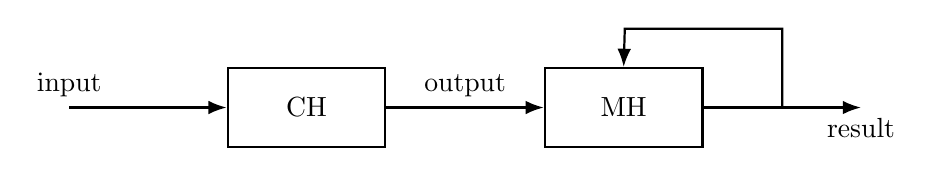
\begin{tikzpicture}[>=Latex, node distance=2cm, thick]

  \node[draw, minimum width=2cm, minimum height=1cm, align=center] (CH) {CH};
  \node[draw, minimum width=2cm, minimum height=1cm, align=center, right=of CH] (MH) {MH};

  \draw[->] ($(CH.west)+(-2,0)$) -- (CH.west) node[pos=0, above] {input};
  
  \draw[->] (CH.east) -- (MH.west) node[midway, above] {output};

  \draw[->] (MH.east) -- ++(1,0) -- ++(0,1) -- ++(-2,0) -- (MH.north);      

  \draw[->] (MH.east) -- ++(2,0) node[pos=1, below] {result};

\end{tikzpicture}
    \caption{Heuristic solution}
    \label{fig:solution}
\end{figure}

The Algorithm designed to solve this problem is a heuristic solution that will be made out of a Construction Hieuristic $(C\!H)$ that produces a starting point based on pre-defined constraints, that feeds into a Meta Heuristic $(M\!H)$ that finds a better solution starting from the output of the construction heuristic and self-improving until an acceptable result is returned. 


\section{Complementing the Heuristic Approach using Machine Learning}
Due to the fact that management workers today place the items manually using tacit knowledge that they have accumulated over the years, then what this thesis proposes is to emulate that same knowledge by learning which placement patterns tend to work together and which do not.

The idea is that if they have knowledge of an adequate solution from the get-go with some risk of overlap, then we can train a Deep Learning Model $(M\!L)$ on such previous data to give the algorithm a better starting point, thus (in theory) reducing the runtime of that algorithm.

\begin{figure}[ht]
    \centering
    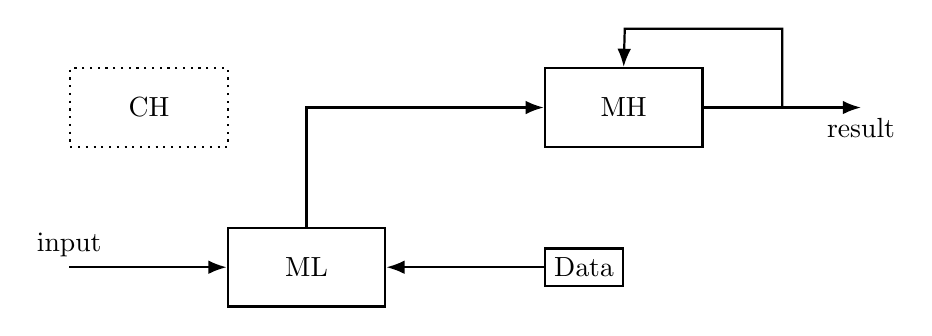
\begin{tikzpicture}[>=Latex, node distance=2cm, thick]
        \node[draw, minimum width=2cm, minimum height=1cm, align=center] (MH) {MH};
\node[draw, minimum width=2cm, minimum height=1cm, below left=1cm and 2cm of MH] (ML) {ML};
        \node[draw, align=center, right=of ML] (Data) {Data};
        \node[draw, dotted, minimum width=2cm, minimum height=1cm, align=center, left=4cm of MH] (CH) {CH};
        \draw[->] (MH.east) -- ++(1,0) -- ++(0,1) -- ++(-2,0) -- (MH.north);      

        \draw[->] (MH.east) -- ++(2,0) node[pos=1, below] {result};

        \draw[->] ($(ML.west)+(-2,0)$) -- (ML.west) node[pos=0, above] {input};

        \draw[->] (Data.west) -- (ML.east);

        \draw[->] (ML.north) |- (MH.west);

    \end{tikzpicture}
    \caption{ML solution}
    \label{fig:ml_solution}
\end{figure}

However it is worth to consider that such an approach can prove redundant or yield worse results if the problem at hand is an easy problem where many solutions can be found quickly, as opposed to a hard problem where a desired solution may not even be found. 

\section{JSON to Vector Methodology}
Machine learning models operate on numerical vector data, often represented as \textit{tensors}, rather than on raw JSON structures. Given a list of JSON objects on an assembly line, each JSON can be encoded into a fixed-length vector $x_t$ by extracting and normalizing its features. This process transforms the entire list into a sequence of vectors ${[x_1, x_2, \dots, x_N]}$. Using sequences from historical data, a model can then be trained to learn a mapping from an input order of JSONs to a desired output order.

\section{System Architecture}

The system will be implemented using PyTorch. Historical assembly line data will serve as input to the machine learning model, but this data must first be vectorized, as most ML frameworks, including PyTorch, operate on numerical vectors rather than structured formats like JSON.

The model architecture is inspired by sequence-to-sequence (Seq2Seq) models, which are commonly used in language processing tasks, such as machine translation. However, the traditional Seq2Seq architecture must be adapted to handle mixed-model sequencing rather than natural language. One challenge is that Seq2Seq models have a tendency to repeat “safe” tokens; in the context of a Mixed-Model Assembly Line (MMAL), this could manifest as repeatedly placing the easiest product in the sequence. To address this, constraints will be added to prevent repetition and encourage diverse permutations.  

Alternative architectures, such as Transformer networks or Pointer Networks, will also be explored to determine the most effective approach for sequencing tasks.  

To evaluate model performance before using historical data, a set of synthetic “puzzles” will be created. These puzzles will be scrambled product sequences with known solutions, allowing the model to learn placement strategies in a controlled environment. After successful training on these synthetic sequences, the model will be tested on real historical data to assess its ability to generalize to practical assembly line scenarios.

Finally, once trained, the model parameters will be stored to avoid retraining for each new sequence, ensuring the system can provide predictions efficiently during production.

  % Pytorch, We'll take historical assembly line data and feed the data into the machine learning algorithm, but to do that we must first vectorize it as ML handles vectors rather than json. Also the format for the historical data is probably json.  
  % Because Seq2Seq traditionally is used for language based tasks, like translation from one language to another, the model might have to be reworked so that it can process mixed model sequencing.
    % Pointer networks could be worth to take a look at. 
    % When the model is trained we must find a way to store the adjusted values of the nn so that we don't have to train it each and every time. DONE!
   %Seq2Seq is flawed in the fact that it has a habit of reusing safe tokens, in a sentence it might continously write "the" as it is a common word in english. In the case of the MMAL it instead repeats the "easiest" product, so a constraint has to be made which will effectively prevent repetition and force permutation placements. Alternatively we investigate alternative model types, such as transformer networks or pointer networks.
   % Creating puzzlepieces - In order to find out which model that is the best before attempting with any previous data I first propose that I create a puzzle and scramble it for the machine to attempt solving. I will of course throw in the correct solutions as training data and then eventually give it some scrambled puzzles to see if it figures it out.

\section{Transforming a language-based model into a sequence based model}

The models examined in this thesis were originally designed for natural language processing tasks, such as translation between languages. Both sequence-to-sequence and transformer-based architectures rely on a predefined vocabulary. This raises the question of whether a list of products can be treated analogously to a collection of words where each product variation forms a distinct element within the vocabulary. Doing so could allow the model to more accurately replicate historical data, along with its flaws.

However, certain constraints must be imposed as language models often overproduce common tokens such as “the,” since these words are statistically more likely to appear in most positions in any given English sentence. To avoid this bias, the model must instead operate on genuine rearrangements or permutations relevant to our specific application.

\subsection{The Tokenizer}
    As one may expect when working with models designed for language, we find that most ready-made tokenizers are made to handle words in natural sentences rather than json-data or vectorized data. One way to circumvent this hurdle is to simply flatten the JSON data so that it becomes a sequence of numerical data -- a string!

\begin{figure}[ht]
    \centering
    \vspace{0.5cm}

    \begin{tikzpicture}[
        json/.style={inner sep=6pt, align=left, font=\ttfamily\small},
        arrow/.style={thick, -{Stealth[length=3mm, width=2mm]}}
    ]

    \node[json] (orig) {
    \{\\
    \quad "id": $n$,\\
    \quad "data": \{\\
    \quad\quad "s1": $x$,\\
    \quad\quad "s2": $y$,\\
    \quad\quad ...\\
    \quad\quad "$s_n$": $z$\\
    \quad\}\\
    \}\\
    };

    \node[json, right=2.5cm of orig] (flat) {
         "id: $n$, s1: $x$, s2: $y$, \dots, $s_n$: $z$"
    };

    % Arrow
    \draw[arrow] (orig.east) -- (flat.west);

    \end{tikzpicture}

    \vspace{0.5cm}
    \caption{Pre-processing JSON data by flattening nested fields.}
    \label{fig:flatten}
\end{figure}

\subsection{Training the Model}
Most of the models explored in this thesis are traditionally applied to translation tasks, where the goal is to map text from one language to another. The training data in such a case might look like:

\vspace{0.5cm}

[sv: "Jag glömde min plånbok", en: "I forgot my wallet"]

\vspace{0.5cm}

Which will allow the model to learn how a sentence in the source language corresponds to one in the target language. 

In our case, the challenge is different as we're not dealing with linguistic sequences or semantic transformations. Instead, our objective is to learn how to \textit{rearrange} items rather than generating new content. 

If we take a look at how Large Language Models are trained, we see that they are exposed to vast amounts of text data and learn statistical relationships between tokens through iterative training. By analogy, we can train a model on large sets of structured examples to learn how to map one ordering of items to another. With appropriate constraints or loss functions to enforce rearrangement behavior, this approach provides a viable framework for our training objective.



\chapter{Experiments and results}
\section{Dataset}
We did get an official dataset from a production run, the dataset however contained a few issues that had to be resolved.
\subsection{Fitting the data}
    The data we got contained everything we needed to visualize it on a timeline similar to \autoref{fig:assembly} where timeslots had to be manually offset to better fit between allocations. The algorithm to fit the alloctions was: [blablabla] with the following criteria: [blablabla]. The reason that the data needed additional processing was due to the fact that some allocations exceeded the given 700 cmin window, and needed to borrow time from neighbouring stations.

    Without offsetting any timeslots roughly 2,000 overlaps were found.
    
    After processing the data we were left with 300. %Lies, plz fix
\section{Evaluation Metrics}
\section{Runtime Analysis}

\chapter{Discussion}
\section{Interpretation of Results}
\section{Limitations}
    As is the case in many machine learning projects the lack of data to train on led to the downfall of this project.
\section{Future Work}


\begin{thebibliography}{99}
\bibitem{ref1}
J. Abbasi, \textit{Predictive Maintenance in Industrial Machinery using Machine Learning}, 
Master’s thesis, Luleå University of Technology, Department of Computer Science, Electrical and Space Engineering, 2021.
\bibitem{ref2}
A. Dupuis, C. Dadouchi, and B. Agard, 
        \textit{A decision support system for sequencing production in the manufacturing industry},
\textit{Computers \& Industrial Engineering}, vol.~185, p.~109686, 2023. 
\bibitem{ref3} J. Lindén, 
    \textit{Understand and Utilise Unformatted Text Documents by Natural Language Processing Algorithms}, 
    Master’s thesis, Mid Sweden University, Department of Information and Communication Systems (IST), Spring 2017.
\bibitem{ref4} Ian Pointer,
\textit{Programming PyTorch for Deep Learning},
O'Reilly Media, 2019.
\bibitem{ref5} 
A. Vaswani, N. Shazeer, N. Parmar, J. Uszkoreit, L. Jones, 
A. N. Gomez, Ł. Kaiser, and I. Polosukhin, 
\textit{Attention is All You Need}, Advances in Neural Information Processing Systems (NeurIPS), vol.~30, 2017.
\bibitem{ref6} 
C. Fink, O. Schelén, and U. Bodin, 
\textit{Work in progress: Decision support system for rescheduling blocked orders}, 
Department of Computer Science, Electrical and Space Engineering, Luleå University of Technology, 2023.
\bibitem{ref7} O. Vinyals, M. Fortunato, and N. Jaitly, 
    \textit{Pointer Networks}, 
    Department of Mathematics, University of California Berkeley, 2015.
\bibitem{refx} Author, Title, Journal, Year.
\end{thebibliography}
\end{document}
